\documentclass[11pt,a4paper]{article}

\usepackage[margin=2.2cm]{geometry}
\usepackage{amsmath,amssymb}
\usepackage{booktabs}
\usepackage{graphicx}
\usepackage{caption}
\usepackage{float}
\usepackage{siunitx}
\DeclareSIUnit{\GeV}{\giga\electronvolt}
\DeclareSIUnit{\TeV}{\tera\electronvolt}
\DeclareSIUnit{\keV}{\kilo\electronvolt}
\DeclareSIUnit{\ns}{\nano\second}
\DeclareSIUnit{\cm}{\centi\metre}
\DeclareSIUnit{\mm}{\milli\metre}
\DeclareSIUnit{\rad}{\radian}
\DeclareSIUnit{\pb}{pb}
\DeclareSIUnit{\fb}{fb}
\usepackage[hidelinks]{hyperref}
\usepackage{microtype}
\usepackage{setspace}
\setstretch{1.08}

\graphicspath{{madgraph_figures/}}

\title{Quirk plane search with MadGraph and Pythia:\\ efficiencies, uncertainties, and Figures 2--5}
\author{Comparison with Knapen, Lou, Papucci, and Setford, arXiv:1708.02243}
\date{}

\begin{document}
\maketitle

\begin{abstract}
This note reports the MadGraph5\_aMC@NLO and Pythia~8 samples of the quirk plane search.
The electroweak sample is Drell--Yan production of an \SI{800}{\GeV} vector-like lepton.
The colored sample is QCD production of an \SI{1800}{\GeV} vector-like quark.
Both use a string scale of \SI{4}{\keV}.
Every cut is counted sequentially.
Each efficiency is given with its binomial standard error and a Wilson 95\% confidence interval, and is compared with Table~I of the paper.
The generator settings are listed in full.
Figures~2--5 of the paper are reproduced for these benchmarks: the internal angular momentum and separation, the rotation of the quirk plane, one event projected onto its reconstructed plane, and the distributions of the thickness \(\Delta s\) and the width \(\Delta w\).
\end{abstract}

\section{Generator settings}
The hard process and the parton shower come from MadGraph5\_aMC@NLO~3.8.0 and Pythia~8.317.
The quirk oscillation is not part of Pythia.
After the shower, each matched event is propagated with the straight-string equation of motion in a \SI{2}{\tesla} solenoid, at \(\Lambda = \SI{4}{\keV}\), and passed through the eight-layer barrel and the plane finder.

\subsection{Collider and run card}
Both processes use the same collider settings.
\begin{center}
\begin{tabular}{ll}
\toprule
Setting & Value \\
\midrule
Beams & proton--proton \\
Beam energy & \SI{6500}{\GeV} each, so \(\sqrt{s} = \SI{13}{\TeV}\) \\
PDF & NNPDF2.3 LO, LHAPDF set \texttt{nn23lo1} \\
Random seed & 170802243 \\
Events requested & 2000 unweighted events \\
Cores & 16 \\
Extra-jet matching & MLM, \texttt{ickkw = 1} \\
Matching scale \(Q_{\mathrm{cut}}\) & \texttt{xqcut = 30}~\si{\GeV} \\
Pythia jet-matching scale & \texttt{JetMatching:qCut = 45}~\si{\GeV} \\
Maximum extra jets & \texttt{JetMatching:nJetMax = 1} \\
Light flavours in the match & \texttt{JetMatching:nQmatch = 4} \\
Jet algorithm & \(k_T\), exclusive, cone radius 1, \texttt{doShowerKt = off} \\
Jet \(p_T\) cut in the matrix element & \texttt{ptj = 10}~\si{\GeV} \\
Scale and PDF systematics & off (\texttt{use\_syst = False}) \\
MadSpin & off \\
Analysis & off \\
\bottomrule
\end{tabular}
\end{center}

\subsection{Electroweak process}
The electroweak quirk is the charge\(-1\) vector-like lepton \texttt{taup} in the model \texttt{VLLS\_NLO}.
Its PDG code is 17 and it is a color singlet.
The mass parameter is \(\texttt{MTAUP} = \SI{800}{\GeV}\).
The width is set to zero by
\(\texttt{epstaupeL} = \texttt{epstaupmuL} = \texttt{epstauptaL} = 0\).
The generated processes are
\begin{align*}
p p &\to \tau'\bar{\tau}', && \texttt{QED=2}, \\
p p &\to \tau'\bar{\tau}'\, j, && \texttt{QED=2},\ \texttt{QCD=1}.
\end{align*}
Hadronization is left at the Pythia default.
The lepton is a color singlet, so there is no QCD string between the pair.
MadGraph reports a parton-level cross section of
\(3.814\times 10^{-4} \pm 1.901\times 10^{-6}\)~\si{\pb}
for 2000 events.
MLM matching keeps 1040 events.
The matched cross section is
\(1.983\times 10^{-4} \pm 4.374\times 10^{-6}\)~\si{\pb}.
The efficiencies below use these 1040 matched events as \(N_{\mathrm{gen}}\).

\subsection{Colored process}
The colored quirk is the charge \(+2/3\) vector-like quark \texttt{tp} in the model \texttt{VLQ\_UFO}.
Its PDG code is 6000006 and it is a color triplet.
The mass parameter is \(\texttt{MTP} = \SI{1800}{\GeV}\) and the width is \(\texttt{WTP} = 0\).
The generated processes are
\begin{align*}
p p &\to t' \bar t', \\
p p &\to t' \bar t' j.
\end{align*}
Pythia hadronization is switched off with \texttt{HadronLevel:all = off}.
A stable colored pair does not leave enough energy for a QCD string to fragment, and with hadronization left on the shower never writes an event.
The dark string is the straight-string propagator in this package, not the Pythia string.
The parton shower and the MLM match are still performed.
MadGraph reports a parton-level cross section of
\(7.566\times 10^{-4} \pm 3.700\times 10^{-6}\)~\si{\pb}
for 2000 events.
MLM matching keeps 855 events.
The matched cross section is
\(3.234\times 10^{-4} \pm 8.518\times 10^{-6}\)~\si{\pb}.
The efficiencies below use these 855 matched events as \(N_{\mathrm{gen}}\).

These two models are vector-like fermions used as proxies for the quirk.
Their cross sections are the MadGraph results for those models.
They are not the quirk cross sections used for the discovery contours in the paper.
The JSON files also contain a field \texttt{cross\_section\_pb} from an earlier toy estimate.
That field is not the MadGraph cross section and is not used in this note.

\subsection{Quirk propagation and the detector}
Each matched event supplies the two heavy-fermion three-momenta.
The pair is started at the origin with a separation of \(10^{-3}\)~\si{\mm} along the relative velocity.
The straight-string force and the Lorentz force are integrated in a \SI{2}{\tesla} field along \(z\), until both quirks leave the outer barrel or \SI{25}{\ns} have passed.
Hits are measured relative to that vertex.
The \SI{45}{\mm} beam spot is not sampled again on top of the MadGraph event.
Pixel hits are moved to the pixel centre: \SI{50}{\micro\metre} in \(r\phi\), \SI{0.25}{\mm} in \(z\) on the innermost layer and \SI{0.40}{\mm} on the other pixel layers.
SCT hits are smeared by \SI{34}{\micro\metre} in \(r\phi\), twice the \SI{17}{\micro\metre} intrinsic resolution.
The SCT stereo \(z\) uncertainty is about \SI{1}{\mm}.
It is not applied as a shift of the hit, because it is larger than the \SI{0.1}{\mm} thickness cut.
Neighboring hits are merged.
No pileup and no photon conversions are overlaid on these samples.
The colored charged-hadron fraction of 30\% is not applied inside the efficiency.
It is used only when a yield is quoted.

\section{Efficiency definitions}
An event is counted at a cut only if it has passed every earlier cut.
The three efficiencies in the paper are ratios of those counts,
\begin{align}
\varepsilon_{\mathrm{trig}}
  &= \frac{N_{\mathrm{trig}}}{N_{\mathrm{gen}}},
  &
  N_{\mathrm{trig}}
  &= \#\{p_T > \SI{200}{\GeV}\},
  \label{eq:trig}
  \\
\varepsilon_{\mathrm{fid}}
  &= \frac{N_{\mathrm{fid}}}{N_{\mathrm{trig}}},
  \label{eq:fid}
  \\
\varepsilon_{\mathrm{reco}}
  &= \frac{N_{\mathrm{reco}}}{N_{\mathrm{fid}}},
  \label{eq:reco}
  \\
\varepsilon
  &= \varepsilon_{\mathrm{trig}}\,
     \varepsilon_{\mathrm{fid}}\,
     \varepsilon_{\mathrm{reco}}
   = \frac{N_{\mathrm{reco}}}{N_{\mathrm{gen}}}.
  \label{eq:total}
\end{align}
Here \(N_{\mathrm{gen}}\) is the number of events kept by MLM matching, 1040 for the electroweak sample and 855 for the colored sample.
The fiducial count \(N_{\mathrm{fid}}\) requires both quirks to intersect all eight barrel layers, with every hit time below \SI{25}{\ns}.
The reconstruction count \(N_{\mathrm{reco}}\) is the number of events that pass the final hit-pattern cut.
Because the flow is sequential, that count already requires the trigger, the fiducial requirement, the seed windows, the factor-of-three growth test, \(\Delta w < \SI{1}{\cm}\), and \(\Delta s < \SI{0.01}{\cm}\).

The individual cuts, in order, are:
\begin{enumerate}
\item \textbf{Generated.} Every matched event.
\item \textbf{Trigger.} Pair transverse momentum above \SI{200}{\GeV}.
\item \textbf{Fiducial.} Both quirks hit all eight layers within \SI{25}{\ns}.
\item \textbf{Layer-8 seed.} A hit pair on layer 8 with \(\Delta\phi < 0.1\) and \(\Delta z < \SI{2}{\cm}\).
\item \textbf{Layer-7 seed.} A hit pair on layer 7 in the same window.
\item \textbf{Seed prefilter.} The two pairs agree within \SI{0.5}{\rad} and \SI{80}{\mm}. This removes combinations that cannot satisfy the \SI{1}{\cm} width cut.
\item \textbf{Seed thickness.} The four seed hits have \(\Delta s < \SI{0.05}{\cm}\).
\item \textbf{Seed width.} The four seed hits have \(\Delta w < \SI{1}{\cm}\).
\item \textbf{Forward direction.} Every seed hit satisfies \(\boldsymbol{n}_3\cdot\boldsymbol{x} > 0\).
\item \textbf{Inward walk.} From layer 6 down to layer 1, a hit is added only when both \(\Delta s\) and \(\Delta w\) stay within a factor of three of their current values, and the finished plane has \(\Delta w < \SI{1}{\cm}\).
\item \textbf{Final thickness.} The finished plane has \(\Delta s < \SI{0.01}{\cm}\).
\item \textbf{Hit pattern.} Seven layers contain two hits and the remaining layer contains at least one.
\end{enumerate}

\section{Wilson intervals}
Each efficiency is a binomial proportion \(k/n\), with estimate \(\hat{p} = k/n\).
The standard error is
\begin{equation}
\sigma = \sqrt{\frac{\hat{p}\,(1-\hat{p})}{n}}.
\label{eq:se}
\end{equation}
The 95\% interval is the Wilson score interval. With \(z = 1.960\),
\begin{equation}
\begin{aligned}
\hat{p}_{\mathrm{W}}
&=
\left(\hat{p} + \frac{z^{2}}{2n}\right)
\frac{1}{1 + z^{2}/n},
\\
\delta
&=
\frac{z}{1 + z^{2}/n}
\sqrt{
  \frac{\hat{p}\,(1-\hat{p})}{n}
  + \frac{z^{2}}{4n^{2}}
},
\end{aligned}
\label{eq:wilson}
\end{equation}
and the interval is \(\hat{p}_{\mathrm{W}} \pm \delta\), clipped to \([0,1]\).
For a conditional cut, \(k\) is the number of events that pass the cut and \(n\) is the number that reached it.
The paper does not quote uncertainties on Table~I.

\section{Electroweak sample}
\label{sec:ew}
Mass \SI{800}{\GeV}, string scale \SI{4}{\keV}, \(N_{\mathrm{gen}} = 1040\) matched events.

\begin{table}[H]
\centering
\caption{Sequential cut flow for the electroweak MadGraph sample. The efficiency is \(k/n\), where \(n\) is the number of events that reached the cut.}
\label{tab:ew-cuts}
\small
\begin{tabular}{lrrrrr}
\toprule
Cut & \(N_{\mathrm{pass}}\) & \(N_{\mathrm{in}}\) & Efficiency & Std.\ error & Wilson 95\% CI \\
\midrule
Generated & 1040 & 1040 & 1.000 & 0.000 & [1.000, 1.000] \\
Trigger & 182 & 1040 & 0.175 & 0.012 & [0.153, 0.199] \\
Fiducial & 58 & 182 & 0.319 & 0.035 & [0.255, 0.390] \\
Layer-8 seed & 53 & 58 & 0.914 & 0.037 & [0.814, 0.963] \\
Layer-7 seed & 51 & 53 & 0.962 & 0.026 & [0.872, 0.990] \\
Seed prefilter & 40 & 51 & 0.784 & 0.058 & [0.654, 0.875] \\
Seed \(\Delta s\) & 40 & 40 & 1.000 & 0.000 & [0.912, 1.000] \\
Seed \(\Delta w\) & 40 & 40 & 1.000 & 0.000 & [0.912, 1.000] \\
Forward & 40 & 40 & 1.000 & 0.000 & [0.912, 1.000] \\
Inward walk & 40 & 40 & 1.000 & 0.000 & [0.912, 1.000] \\
Final \(\Delta s\) & 39 & 40 & 0.975 & 0.025 & [0.871, 0.996] \\
Hit pattern & 22 & 39 & 0.564 & 0.079 & [0.410, 0.707] \\
\bottomrule
\end{tabular}
\end{table}

\begin{table}[H]
\centering
\caption{Electroweak efficiencies as defined in Eqs.~\eqref{eq:trig}--\eqref{eq:total}.}
\label{tab:ew-eff}
\begin{tabular}{lrrrr}
\toprule
Efficiency & Count & Estimate & Std.\ error & Wilson 95\% CI \\
\midrule
\(\varepsilon_{\mathrm{trig}}\) & $182/1040$ & 0.175 & 0.012 & [0.153, 0.199] \\
\(\varepsilon_{\mathrm{fid}}\) & $58/182$ & 0.319 & 0.035 & [0.255, 0.390] \\
\(\varepsilon_{\mathrm{reco}}\) & $22/58$ & 0.379 & 0.064 & [0.266, 0.508] \\
\(\varepsilon\) & $22/1040$ & 0.021 & 0.004 & [0.014, 0.032] \\
\bottomrule
\end{tabular}
\end{table}

The last row of Table~\ref{tab:ew-cuts} is not \(\varepsilon_{\mathrm{reco}}\).
It is the hit-pattern efficiency among events that already passed the final \(\Delta s\) cut.
The paper's reconstruction efficiency uses the fiducial sample as the denominator.

\section{Colored sample}
\label{sec:qcd}
Mass \SI{1800}{\GeV}, string scale \SI{4}{\keV}, \(N_{\mathrm{gen}} = 855\) matched events.

\begin{table}[H]
\centering
\caption{Sequential cut flow for the colored MadGraph sample.}
\label{tab:qcd-cuts}
\small
\begin{tabular}{lrrrrr}
\toprule
Cut & \(N_{\mathrm{pass}}\) & \(N_{\mathrm{in}}\) & Efficiency & Std.\ error & Wilson 95\% CI \\
\midrule
Generated & 855 & 855 & 1.000 & 0.000 & [1.000, 1.000] \\
Trigger & 208 & 855 & 0.243 & 0.015 & [0.216, 0.273] \\
Fiducial & 54 & 208 & 0.260 & 0.030 & [0.205, 0.323] \\
Layer-8 seed & 50 & 54 & 0.926 & 0.036 & [0.824, 0.971] \\
Layer-7 seed & 48 & 50 & 0.960 & 0.028 & [0.865, 0.989] \\
Seed prefilter & 43 & 48 & 0.896 & 0.044 & [0.778, 0.955] \\
Seed \(\Delta s\) & 43 & 43 & 1.000 & 0.000 & [0.918, 1.000] \\
Seed \(\Delta w\) & 43 & 43 & 1.000 & 0.000 & [0.918, 1.000] \\
Forward & 43 & 43 & 1.000 & 0.000 & [0.918, 1.000] \\
Inward walk & 43 & 43 & 1.000 & 0.000 & [0.918, 1.000] \\
Final \(\Delta s\) & 43 & 43 & 1.000 & 0.000 & [0.918, 1.000] \\
Hit pattern & 29 & 43 & 0.674 & 0.071 & [0.525, 0.795] \\
\bottomrule
\end{tabular}
\end{table}

\begin{table}[H]
\centering
\caption{Colored efficiencies as defined in Eqs.~\eqref{eq:trig}--\eqref{eq:total}.}
\label{tab:qcd-eff}
\begin{tabular}{lrrrr}
\toprule
Efficiency & Count & Estimate & Std.\ error & Wilson 95\% CI \\
\midrule
\(\varepsilon_{\mathrm{trig}}\) & $208/855$ & 0.243 & 0.015 & [0.216, 0.273] \\
\(\varepsilon_{\mathrm{fid}}\) & $54/208$ & 0.260 & 0.030 & [0.205, 0.323] \\
\(\varepsilon_{\mathrm{reco}}\) & $29/54$ & 0.537 & 0.068 & [0.406, 0.663] \\
\(\varepsilon\) & $29/855$ & 0.034 & 0.006 & [0.024, 0.048] \\
\bottomrule
\end{tabular}
\end{table}

\section{Comparison with Table~I}
Table~I of arXiv:1708.02243 gives \(\varepsilon_{\mathrm{trig}} = 0.10\) and \(\varepsilon_{\mathrm{fid}} = 0.28\) for the \SI{800}{\GeV} electroweak benchmark, independent of \(\Lambda\), and \(\varepsilon_{\mathrm{reco}} = 0.72\) at \(\Lambda = \SI{4}{\keV}\).
For the \SI{1800}{\GeV} colored benchmark it gives \(\varepsilon_{\mathrm{trig}} = 0.24\) and \(\varepsilon_{\mathrm{fid}} = 0.28\).
It does not list a colored reconstruction efficiency at \SI{4}{\keV}.
The neighboring colored entries are \(\varepsilon_{\mathrm{reco}} = 0.59\) at \SI{3}{\keV} and \(\varepsilon_{\mathrm{reco}} = 0.74\) at \SI{5}{\keV}.

\begin{table}[H]
\centering
\caption{Table~I compared with the MadGraph samples. A Table~I value is marked outside when it does not lie in the Wilson 95\% interval.}
\label{tab:compare}
\footnotesize
\resizebox{\textwidth}{!}{%
\begin{tabular}{llp{4.6cm}rrll}
\toprule
Sample & Efficiency & Table~I & This work & Std.\ error & Wilson 95\% CI & Interval \\
\midrule
Electroweak & \(\varepsilon_{\mathrm{trig}}\) & 0.10 & 0.175 & 0.012 & [0.153, 0.199] & outside \\
Electroweak & \(\varepsilon_{\mathrm{fid}}\) & 0.28 & 0.319 & 0.035 & [0.255, 0.390] & inside \\
Electroweak & \(\varepsilon_{\mathrm{reco}}\) & 0.72 & 0.379 & 0.064 & [0.266, 0.508] & outside \\
Colored & \(\varepsilon_{\mathrm{trig}}\) & 0.24 & 0.243 & 0.015 & [0.216, 0.273] & inside \\
Colored & \(\varepsilon_{\mathrm{fid}}\) & 0.28 & 0.260 & 0.030 & [0.205, 0.323] & inside \\
Colored & \(\varepsilon_{\mathrm{reco}}\) & 0.59 at \SI{3}{\keV}; 0.74 at \SI{5}{\keV} & 0.537 & 0.068 & [0.406, 0.663] & not tabulated at 4 keV \\
\bottomrule
\end{tabular}}
\end{table}

The colored trigger efficiency and both fiducial efficiencies agree with Table~I: each Table~I value lies inside the Wilson interval.
The electroweak trigger efficiency is higher than 0.10, and 0.10 lies outside the interval.
The vector-like lepton model, with one extra jet and MLM matching, is not the same matrix element as the quirk model used for Table~I, so the momentum distribution is not expected to match that entry exactly.
The electroweak reconstruction efficiency is \(22/58\).
The Table~I value 0.72 lies outside its Wilson interval.
The colored reconstruction efficiency at \SI{4}{\keV} is not in Table~I.
Its central value, 0.537, lies below the paper's \SI{3}{\keV} entry of 0.59, and 0.59 lies inside the Wilson interval.
The \SI{5}{\keV} entry 0.74 lies outside that interval.
The fiducial samples that enter \(\varepsilon_{\mathrm{reco}}\) contain 58 and 54 events, so this efficiency is the least precise of the three.

At \SI{300}{\fb^{-1}}, the central matched cross section and the central total efficiency give about \(1.26\) electroweak events.
For the colored sample the same product, multiplied by the 30\% charged fraction, gives about \(0.99\) events.
These yields use the vector-like-fermion cross sections above.
They are not the quirk yields of the paper.

\section{Figures}
\setcounter{figure}{1}
The four figures below correspond to Figures~2--5 of the paper.
Figures~2 and~3 integrate the straight-string equation at the two benchmark masses, \(\Lambda = \SI{4}{\keV}\), in the \SI{2}{\tesla} field.
A showered MadGraph event oscillates many times while its centre of mass crosses the tracker, so those two figures use one resolved trajectory at each benchmark, with the initial conditions stated in the captions.
Figure~4 is reconstructed MadGraph event 192, which has pair \(p_T = \SI{328}{\GeV}\) and passes the hit-pattern cut.
Figure~5 uses every fiducial event in the two matched samples for which the plane finder returned a plane.

\begin{figure}[H]
\centering
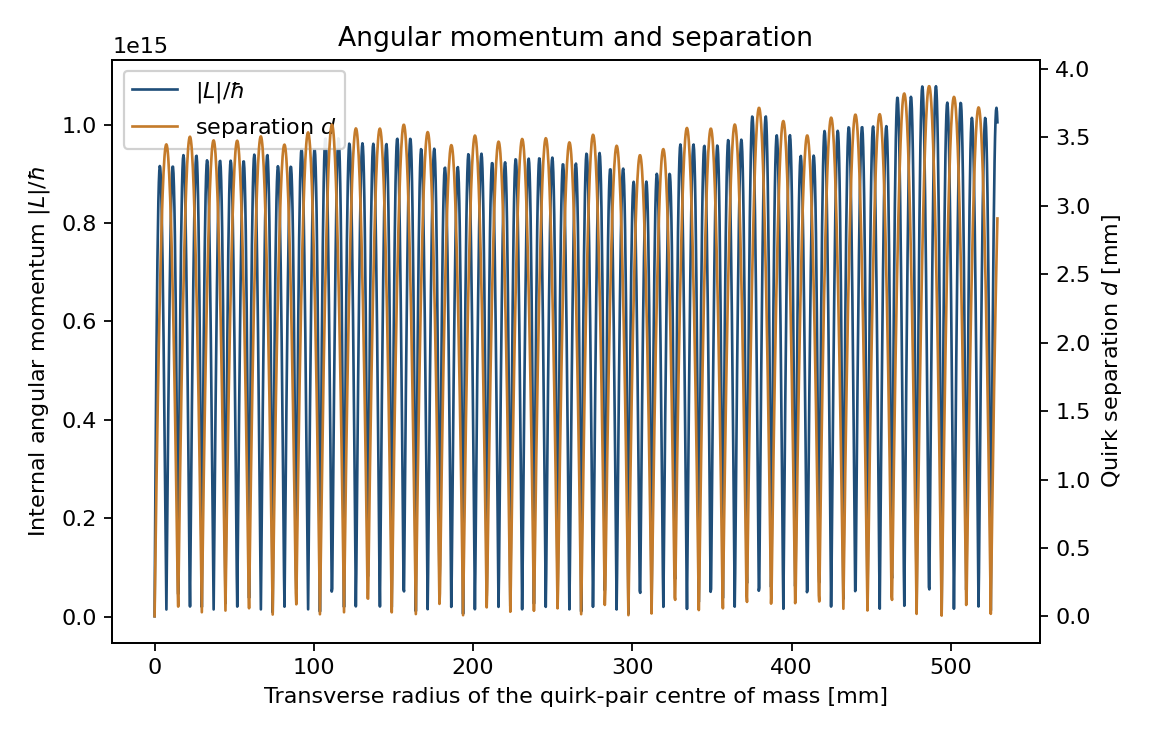
\includegraphics[width=\textwidth]{fig2_angular_momentum.png}
\caption{Internal angular momentum \(|L|/\hbar\) and quirk separation \(d\) versus the transverse radius of the pair centre of mass.
The quirks are produced back to back in their centre of mass with speed \(v = 0.53\) along the axis \((0, 0.2, 1)\), and the pair is boosted by \(\boldsymbol{\beta} = (0.75, 0.05, 0.20)\).
The mass is \SI{800}{\GeV} and the string scale is \SI{4}{\keV}.
On this trajectory \(|L|/\hbar\) reaches \(1.08\times 10^{15}\), and \(d\) runs from \SI{0.001}{\mm} to \SI{3.874}{\mm}.
This is the same pair of quantities as Figure~2 of the paper.}
\label{fig:l}
\end{figure}

\begin{figure}[H]
\centering
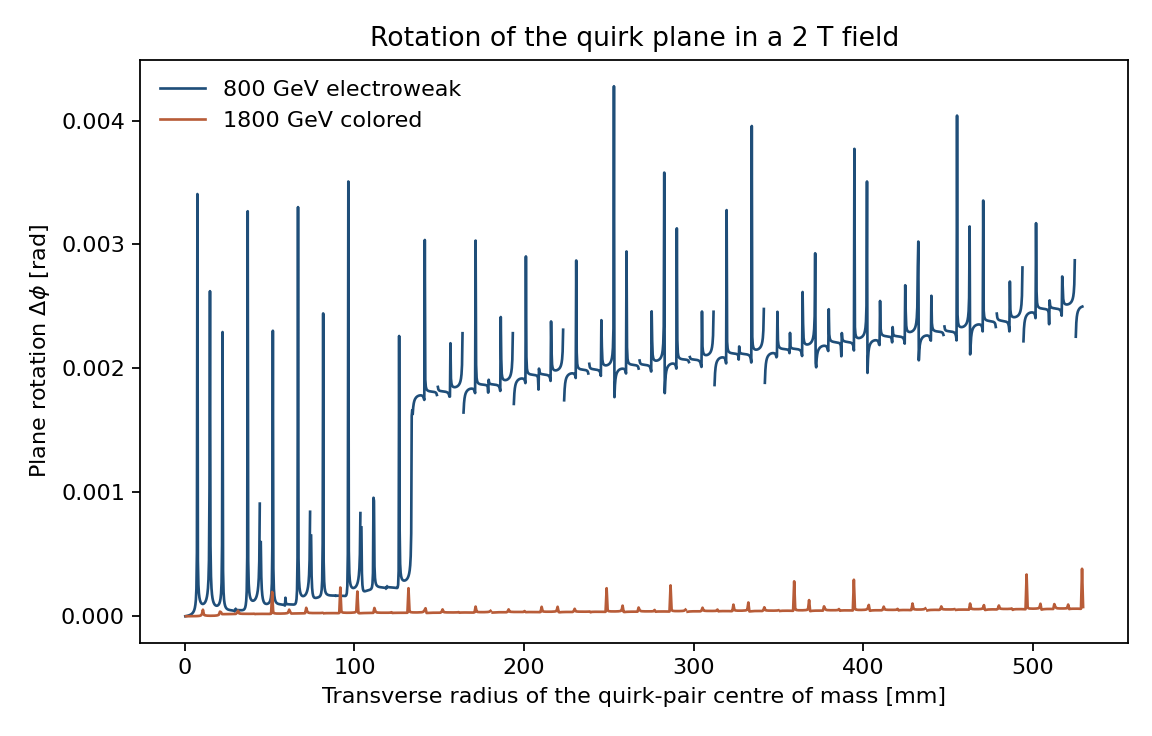
\includegraphics[width=\textwidth]{fig3_plane_rotation.png}
\caption{Angle \(\Delta\phi\) between the instantaneous quirk plane and the plane at the start of the trajectory.
The electroweak curve uses the same initial conditions as Figure~\ref{fig:l} and reaches \(4.28\times 10^{-3}\)~\si{\rad}.
The colored curve has mass \SI{1800}{\GeV}, speed \(v = 0.42\) along \((0.15, 1, 0.1)\), and boost \(\boldsymbol{\beta} = (0.70, 0.10, 0.15)\).
It reaches \(3.83\times 10^{-4}\)~\si{\rad}.
As in Figure~3 of the paper, the rotation remains small compared with the angular size of a tracker hit.}
\label{fig:phi}
\end{figure}

\begin{figure}[H]
\centering
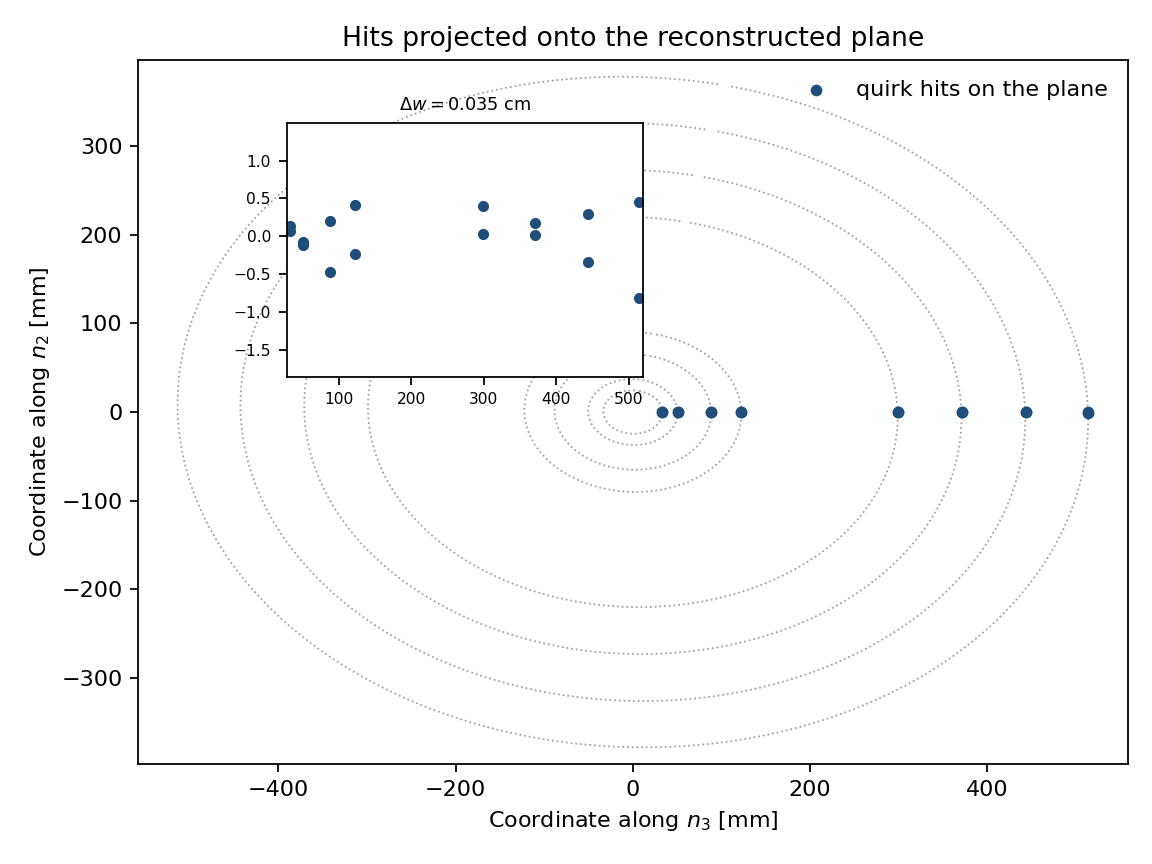
\includegraphics[width=0.92\textwidth]{fig4_plane_projection.png}
\caption{Hits of the electroweak MadGraph event projected onto the reconstructed \((\boldsymbol{n}_3,\boldsymbol{n}_2)\) plane.
The dotted curves are the eight barrel layers.
The fit gives \(\Delta s = \SI{0.0075}{\cm}\) and \(\Delta w = \SI{0.0345}{\cm}\), from 16 hits.
The inset shows the strip, as in Figure~4 of the paper.}
\label{fig:plane}
\end{figure}

\begin{figure}[H]
\centering
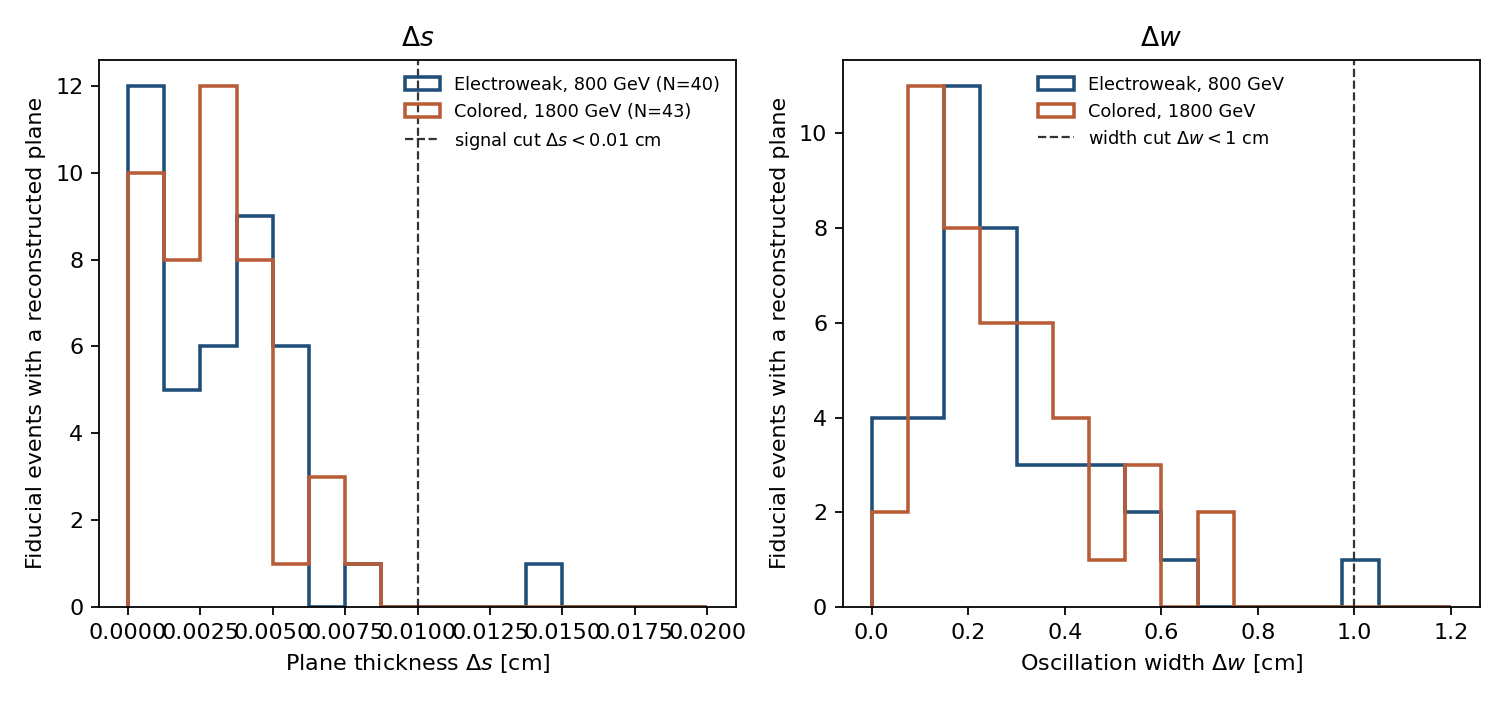
\includegraphics[width=\textwidth]{fig5_delta_s_delta_w.png}
\caption{Thickness \(\Delta s\) and width \(\Delta w\) for fiducial MadGraph events in which the plane finder returned a plane, before the hit-pattern requirement.
The dashed line on the left is the signal cut \(\Delta s < \SI{0.01}{\cm}\).
The dashed line on the right is \(\Delta w < \SI{1}{\cm}\).
There are 40 electroweak events and 43 colored events in the histograms.
Figure~5 of the paper also shows the pileup and photon-conversion background, which was not generated in this run, and its colored curve is at \SI{2}{\keV} rather than \SI{4}{\keV}.}
\label{fig:widths}
\end{figure}

\end{document}
